\documentclass[11pt]{amsbook}
\usepackage{../Ceyhun}
\usepackage{../amsTurkish}
\begin{document}
\hPage{Ceyhun-75}
\begin{equation}
\begin{bmatrix}
0 & D_{12} & ....... & D_{1n} \\
D'_{12} & 0 & ....... & D_{2n} \\
...........& .... & ....... & ...... \\
D'_{1n} & D'_{2n} & ...... & 0 \\
\end{bmatrix}
\end{equation}

bi\c{c}iminde yaz{\i}labilir.

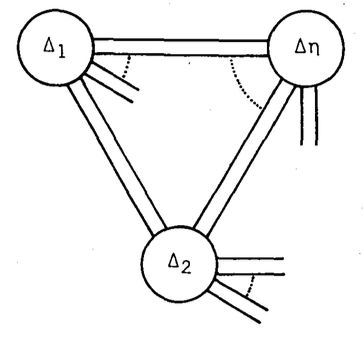
\includegraphics[width=0.75\textwidth,height=0.35\textheight]{images/graph4}

\c{S}ekil 2.4.2 n-k\"{u}meli \c{c}izgenin simgesel g\"{o}sterimi. N-k\"{u}meli \c{c}izgelerin
\"{o}zel bir durumu, iki k\"{u}meli \c{c}izgelerdir.

\begin{definition} 
D\"{u}\u{g}\"{u}mleri iki ba\u{g}{\i}ms{\i}z k\"{u}meye ayr{\i}labilen \c{c}izgelere
\underline{iki k\"{u}meli \c{c}izge} denir.
\end{definition}

\.{I}kik\"{u}meli bir \c{c}(d,a) \c{c}izgesini, k\"{u}melerindeki d\"{u}\u{g}\"{u}mlerin say{\i}s{\i}n{\i} da belirtecek 
bi\c{c}imde \.{I}(m,n) olarak g\"{o}sterece\u{g}iz.
 
\end{document}